\section{Existing platforms}

\subsection{Etherium}
Ethereum is an open blockchain platform that lets anyone build and use decentralised applications that run on blockchain technology. Like Bitcoin, no one controls or owns Ethereum – it is an open-source project \cite{eth_docs}. Ethereum was proposed in late 2013 by Vitalik Buterin, a cryptocurrency researcher and programmer. The system was deployed to production on 30 July 2015

\subsection{Hyperledger}
Hyperledger is an umbrella project of open source blockchain platforms and tools. It was founded in 2016 by Linux foundation with 30 founding members including Accenture, Fujitsu, IBM, Intel \cite{hyperledger_founding}. It was founded these can be used to build a new generation of transactional applications that establishes trust, accountability and transparency at their core while streamlining business processes and legal constraints. Hyperledger incubates handful of business blockchain technologies like distributed ledger frameworks, smart contract engines, client libraries, graphical interfaces. 

\begin{description}
\item[Hyperledger Fabric] is currently the most used private permissioned blockchain solution. It's enterprise-grade, distributed ledger based on blockchain technologies that use smart-contracts to enforce trust between parties that don't trust each other. It was introduced to provide a modular, scalable and secure foundation for industrial blockchain. 
There is a concept of “Channels” where parties that are part of a blockchain can create separate transactions privately and then pass the final state to the be recorded on the main blockchain. This is not unlike state channels in other blockchains, but there is an additional privacy layer.
All participants have known identities, maintained by what Fabric calls “Membership Service Providers” (MSP). If you’re allowing a group of 10 hospitals to participate in your blockchain, each of the 10 hospitals is known to the network. This is the key feature of Hyperledger Fabric that makes it fit well with enterprise solutions.
Consensus: Fabric doesn't use typical Proof of Work or Proof of Stake mechanisms to achieve consensus. Because it’s highly permissioned, it uses a sequence of verified transactions (based on MSP) instead. You can use chain-code to only accept a transaction if two parties who conduct a transaction both sign it and then peers that take in the transaction validate it as well. In short, all we need to worry about for now is that multiple verified participants need to sign transactions for them to get included to the ledger. This is a good fit for enterprise-based blockchains that don’t have a huge number of participants. Because the participants are known to each other, there is a natural deterrent to malicious behaviour \cite{coral_start}. 

Hyperledger Fabric also supports chaincode. Chaincode is the term for programs that run on top of the blockchain to implement the business logic of how applications interact with the ledger. Chaincode typically handles business logic agreed to by members of the network, so it may be considered as a “smart contract”. The state created by a chaincode is scoped exclusively to that chaincode and can’t be accessed directly by another chaincode. Hyperledger Fabric Chaincode APIs implementation is available in Node.js, Golang and Java. Whilst Java support was introduced recently, Node.js and Go lang APIs are quite at a mature level. 

\begin{figure}[H]
    \begin{center}
        \begin{minipage}{\linewidth}
            \begin{center}
                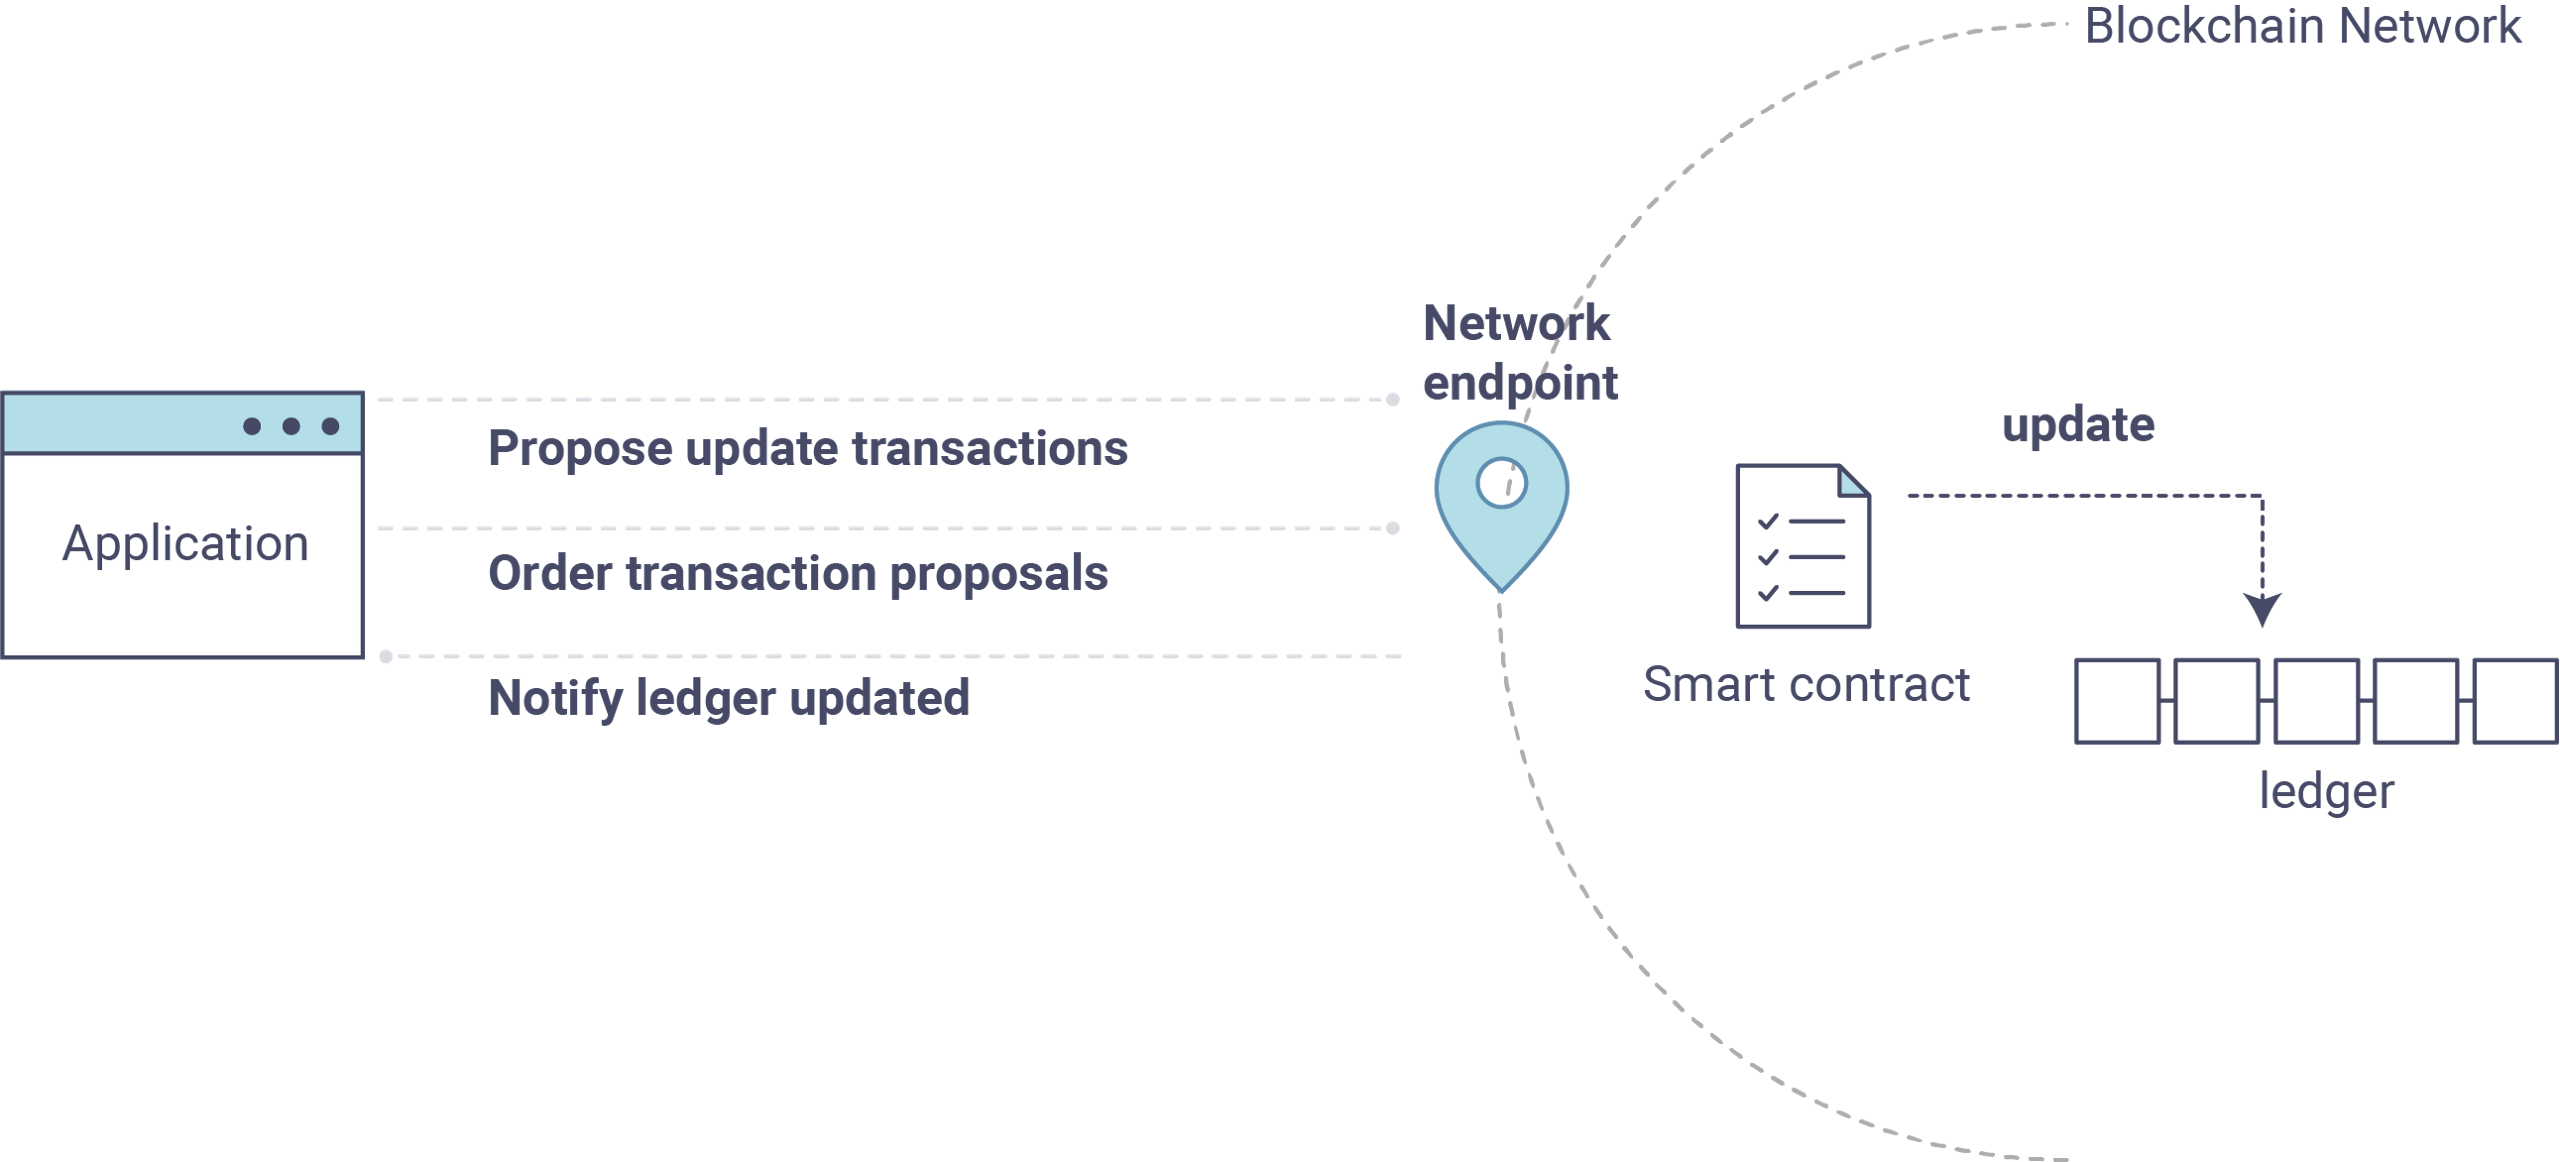
\includegraphics[width=\textwidth,keepaspectratio]{img/chaincode.png}
                \caption{Chaincode diagram}
                \label{obr 1.2.1}
            \end{center}
        \end{minipage}
    \end{center}
\end{figure}


\item[Hyperledger Sawtooth] is an enterprise blockchain platform for building distributed ledger applications and networks. Fabric and Sawtooth share a lot of common features. Main difference roots in Sawtooth support in both permissioned and permissionless blockchain implementation whereas Hyperledger Fabric support only permissioned blockchain implementation. This core difference leads to differences in the consensus algorithm. Since it's private blockchain it' doesn't make any sense to use CPU or GPU power to reach consensus, Sawtooth is using Proof of Elapsed Time (PoET). Similarly to the cryptocurrency network, peers have access to all transaction data.

\item[Hyperledger Composer] is an extensive, open development toolset and framework to make developing blockchain applications easier. The primary goal is to accelerate time to value and make it easier to integrate blockchain applications with the existing business systems. Composer can be used to rapidly develop use cases and deploy a blockchain solution. Composer allows to model business network and integrates existing systems and data with your blockchain applications. Hyperledger Composer supports the existing Hyperledger Fabric blockchain infrastructure and runtime, which supports pluggable blockchain consensus protocols to ensure that transactions are validated according to the policy by the designated business network participants. Composer is used to quickly model the current business network, containing existing assets and the transactions related to them; assets are tangible or intangible goods, services, or property. As part of the business network model we define the transactions which can interact with assets. Business networks also include the participants who interact with them, each of which can be associated with a unique identity, across multiple business networks. \cite{composer}

\item[BigchainDB] is block database with some blockchain characteristics, including decentralization, immutability and native support for assets \cite{bigchaindb}. BigchainDB consists of nodes running BigchainDB Server and related software where each node is controlled by one person or organization. BigchainDB Network is a set of BigchainDB nodes connected to each other to form a BigchainDB network. Each node in the network runs the same software. BigchainDB Consortium are people or organizations that run the nodes in a BigchainDB network belong to a BigchainDB consortium (i.e. another organization). A consortium must have some sort of governance structure to make decisions. If a BigchainDB network is run by a single company, then the “consortium” is just that company. A consortium is an organization which has a BigchainDB network, and where each node in that network has a different operator. As of 2019 BigchainDB is still not ready for production and suitable for mostly for prototyping and experimenting.

\end{description}